\section{Ziel}
Das Ziel dieses Versuches ist es, mithilfe der Ablenkung
eines Elektronenstrahls im elektrischen sowie im transversalen
Magnetfeld bestimmte Eigenschaften zu untersuchen.
Dazu zählen die spezifische Elektronenladung, die Intensität
des Erdmagnetfeldes und die Proportionalität zwischen der
Verschiebung des Leuchtflecks des Elektronenstrahls und der
angelegten Ablenkspannung. Außerdem soll ein Kathodenstrahl-
Oszillograph untersucht werden.

\section{Theorie}
\label{sec:Theorie}
Für beide Versuchsteile wird eine Röhre verwendet, in der ein
Vakuum erzeugt wurde. Dafür wird die so genannte Kathodenstrahlröhre 
bis auf einen Restdruck von ca. $\SI{1e-6}{\milli\bar}$
evakuiert. 

\subsection{Theoretische Grundlage im elektrischen Feld}
%irgendwas hinschreiben

\subsubsection{Aufbau einer Kathodenstrahlröhre}
Die Kathodenstrahlröhre besteht im Wesentlichen aus drei 
Bauteilen (siehe Abb. \ref{fig:roehre}). Zum einen gibt es eine Elektronenkanone, die freie 
Elektronen erzeugt und beschleunigt und in der diese zu einem 
Strahl fokussiert werden. Außerdem gibt es ein Ablenk- und 
ein Nachweissystem.
\begin{figure}
    \centering
    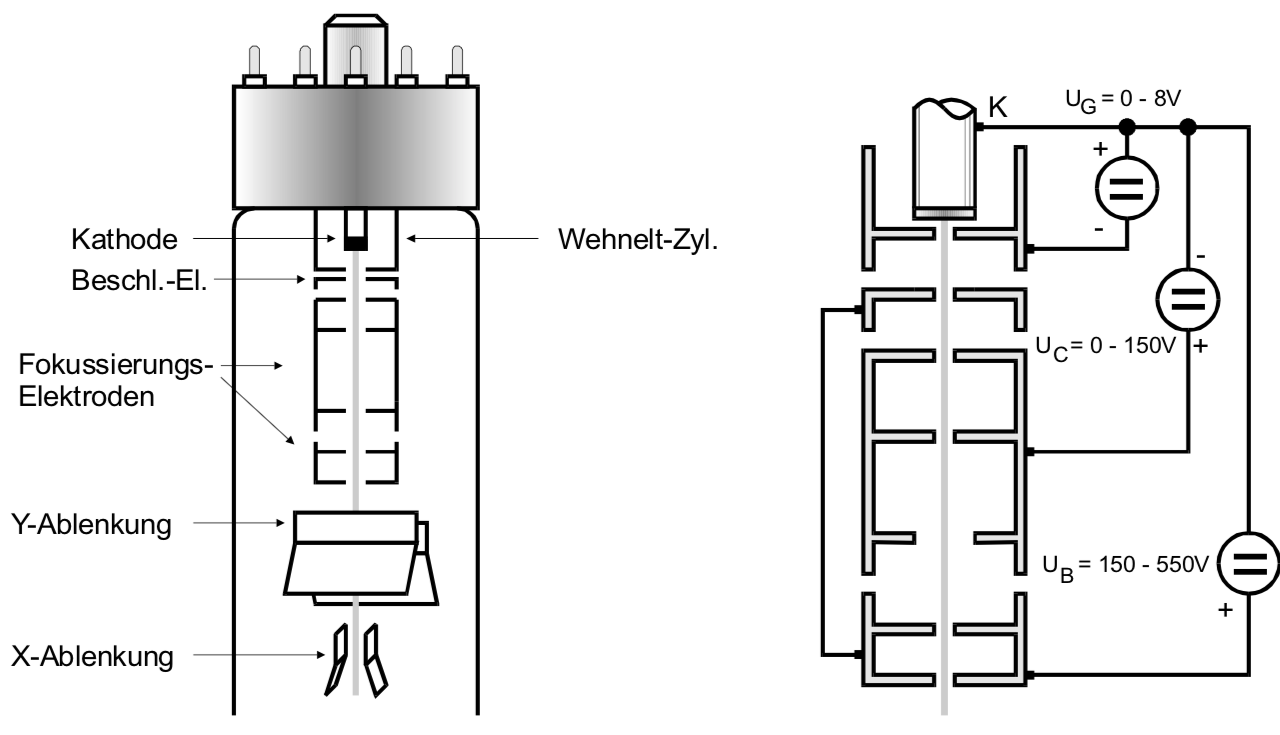
\includegraphics[width=12cm, height=7cm]{build/roehre.png}
    \caption{Der Aufbau einer Kathodenstrahlröhre. \cite{V501}}
    \label{fig:roehre}
\end{figure}

\noindent Die Elektronen werden hierfür durch Glühemission in einem bis zur 
Rotglut erhitzten Draht erzeugt. 
Die Kathode ist von einem Wehnelt-Zylinder umgeben. Mit 
seinem negativen Potential kann die Intensität 
des Elektronenstrahls gesteuert weden. 
Vor dem Zylinder befindet sich eine positiv geladene 
Elektrode, die dafür sorgt, dass sich die freien Elektronen, 
die die Barriere des Zylinders überwinden, auf eine 
Geschwindigkeit $v_\text{z}$ beschleunigen. 
Mit dem Energiesatz ergibt sich dann 
\begin{equation}
    \frac{m_0 \, v_\text{Z}^2}{2} = e_\text{0} \, U_\text{B}.
    \label{eqn:energie}
\end{equation}

\noindent Hinter der Elektrode befinden sich weitere Elektroden, 
die dafür da sind, den Strahl zu fokussieren. Der gebündelte 
Strahl fällt am Ende der Apparatur auf einen Leuchtschirm, 
auf dem die auftreffenden Elektronen die Aktivatorzentren zur 
Emission von Lichtquanten anregen.
Der Leuchtschirm ist mit der Beschleunigungselektrode 
verbunden, sodass er sich nicht negativ laden kann.
Das Ablenksystem besteht aus zwei Plattenpaaren, deren Normalen 
senkrecht aufeinander stehen. Legt man eine Spannung an diese 
Platten an, übt das davon erzeugte $E$-Feld eine Kraft 
auf den Elektronenstrahl aus. 

\subsubsection{Berechnung der Ablenkung eines Elektronenstrahls im elektrischen Feld} %gleiche Überschrift wie in der Anleitung
Die folgenden Gleichungen können in Abb. \ref{fig:roehre2}
grafisch nachvollzogen werden.
\begin{figure}
    \centering
    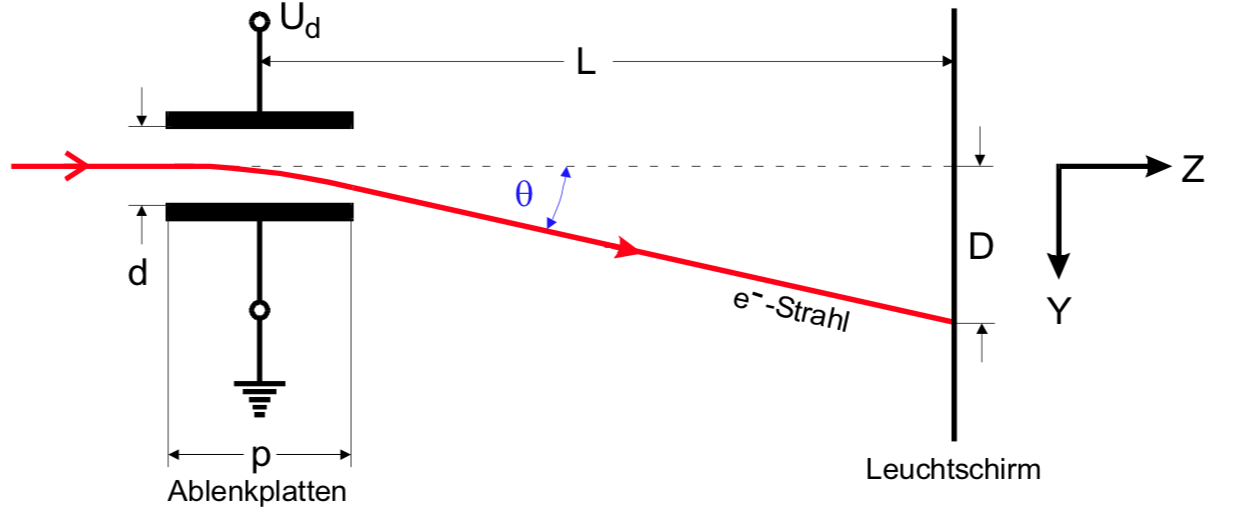
\includegraphics[width=12cm, height=6cm]{build/roehre2.png}
    \caption{Schematische Darstellung der Ablenkung des
    Elektronenstrahls in der Kathodenstrahlröhre. \cite{V501}}
    \label{fig:roehre2}
\end{figure}

\noindent Ist der Plattenabstand $d$ klein gegen die Plattenlänge $p$ 
der Ablenkplatten, kann man annehmen, dass das elektrische 
Feld homogen ist und sich die Feldstärke zu
\begin{equation*}
    E = \frac{U_\text{d}}{d}
\end{equation*} 
ergibt. Auf ein Elektron wirkt dann die entsprechende Kraft, 
die außerhalb der Platten null wird. Diese Kraft ist konstant, 
wodurch sich eine Beschleunigung in $y$-Richtung  
%---> wir haben vorher keine Richtungen erwähnt
ergibt. 
Die erreichte Geschwindigkeit ist 
\begin{equation*}
    v_\text{y} = \frac{e_\text{0}}{m_\text{0}} \frac{U_\text{d}}{d} \Delta t.
\end{equation*}

\noindent Mit der Plattenlänge und der 
gleichförmigen Geschwindigkeit $v_\text{z}$ ergibt sich $\Delta t$ zu
\begin{equation*}
    \Delta t = \frac{p}{v_\text{z}}.
\end{equation*}

\noindent Dieser Ausdruck kann in die vertikale 
Geschwindigkeit $v_\text{y}$ eingesetzt werden. Der Winkel $\theta$ der 
Richtungsänderung setzt sich aus der Division von 
$v_\text{y}$ durch $v_\text{z}$ zusammen. 

\noindent Damit ergibt sich für die Verschiebung $D$ des Leuchtflecks 
\begin{equation*}
    D = L \, \theta = \frac{e_\text{0}}{m_\text{0}} \, L \, \frac{U_\text{d}}{d} \frac{p}{v_\text{z}^2}.
\end{equation*}

\noindent Mit Gleichung \eqref{eqn:energie} ergibt sich dann 
\begin{equation}
    D = \frac{p}{2\, d} \, L \, \frac{U_\text{d}}{U_\text{B}}.
    \label{eqn:leuchtfleck}
\end{equation}

\subsubsection{Der Kathodenstrahl-Oszillograph}
Mit einem Kathodenstrahl-Oszillographen kann die Zeitabhängigkeit
von Wechselspannungen darstellt werden.
Dazu wird an das Plattenpaar, das den Strahl in horizontaler
Richtung ablenkt, eine Sägezahnspannung angelegt. An das Plattenpaar,
das den Strahl vertikal ablenkt, wird die zu untersuchende
Spannung angelegt. Wenn die Synchronisationsbedingung
\begin{equation*}
    n \, \nu_\text{Sä} = m \, \nu_\text{We}
\end{equation*}
erfüllt ist, wird der Verlauf der Wechselspannung auf dem
Leuchtschirm angezeigt.


\subsection{Theoretische Grundlage im magnetischen Feld}
Elektrische Felder üben auf ruhende Ladungen 
eine Kraft aus. Magnetostatische Felder dagegen üben nur auf 
Ladungen, die sich relativ zum Feld bewegen, eine Kraft aus.

\subsubsection{Berechnung der Elektronenbahn im homogenen Magnetfeld}
Eine Ladung $q$, die sich mit der Geschwindigkeit $\vec{v}$ in 
einem homogenen Magnetfeld $\vec{B}$ bewegt, erfährt die Lorentz-Kraft 
\begin{equation}
    \vec{F_\text{L}}= q \, \vec{v} \cross \vec{B}.
    \label{eqn:Lorentz}
\end{equation}

\noindent Die Lorentz-Kraft ist nur nicht null, wenn es eine 
Geschwindigkeitskomponente $\vec{v}$ gibt, die senkrecht zu 
$\vec{B}$ ausgerichtet ist. 

\noindent Das  Magnetfeld ändert allerdings nur die Richtung und ändert 
nicht die Geschwindigkeit. Also ist die Energie konstant 
innerhalb des Systems der Ladung.
%-> E_pot ändert sich nicht -> E_kin konstant -> |vec(v)|=v_0 konstant

\noindent Der Krümmungsradius $r$ der Bahn lässt sich aus dem Gleichgewicht der 
Lorentz- und der Zentrifugalkraft bestimmen. Es ergibt sich 
\begin{equation}
    r= \frac{m_\text{0} \, v_\text{0}}{e_\text{0} \, B}.
    \label{eqn:radius}
\end{equation}
Die rechte Seite der Gleichung ist konstant, insofern ist die 
Krümmungsbahn eine Kreisbahn. 

\subsubsection{Bestimmung der spezifischen Elektronenladung}
Mit Gleichung \ref{eqn:radius} lässt sich die spezifische 
Ladung der Elektronen $e_\text{0}/m_\text{0}$ bestimmen. 
Mit der Beschleunigungsspannung $U_\text{B}$ ergibt sich die 
konstante Geschwindigkeit $v_\text{0}$ zu 
\begin{equation*}
    v_\text{0}= \sqrt{2 \, U_\text{B} \frac{e_\text{0}}{m_\text{0}}}.
\end{equation*}
In einem feldfreien Raum bewegen sich die Elektronen eines 
Kathodenstrahls in Richtung Mittelpunkt des Leuchtschirms und 
erzeugen einen Leuchtfleck. 
Wenn das Magnetfeld eingeschaltet wird, verschiebt sich 
der Leuchtfleck aufgrund der Krümmung auf der vertikalen Achse 
um das Stück $D$. Zwischen dem Wirkungsbereich $L$ (das ist die Weite 
zwischen der Quelle und dem Schirm), dem Stück $D$ und dem 
Radius $r$ ergibt sich über den Satz des Pythagoras die 
Verbindung
\begin{equation*}
    r = \frac{L^2 + D^2}{2D}.
\end{equation*}
Dies kann in \ref{eqn:radius} eingesetzt werden.
Damit ergibt sich der Zusammenhang
\begin{equation}
    \frac{D}{L^2 + D^2}= \frac{1}{\sqrt{8 \, U_\text{B}}}\sqrt{\frac{e_\text{0}}{m_\text{0}}} B.
    \label{eqn:Ende}
\end{equation}

\subsubsection{Das Helmholtz-Spulenpaar}
Ein Helmholtz-Spulenpaar kann ein homogenes Magnetfeld erzeugen.
Der Radius $R$ beider Spulen entspricht dem Spulenabstand.
Die Windungszahl $N$ der Spulen ist ebenfalls identisch.
Im Mittelpunkt ist die Flussdichte $B$ durch
\begin{equation}
    B = \mu_0 \, \frac{8}{\sqrt{125}} \, \frac{N \, I}{R}
    \label{eqn:helmholtz}
\end{equation}
gegeben.

\subsubsection{Erdmagnetfeld}
Die Totalintensität des Erdmagnetfelds ergibt sich mit der horizontal Komponente $B_\text{horizontal}$ und dem Winkel $\varphi$ zu %horizontal oder vertikal und wie heißt der Winkel 
\begin{equation}
    B_\text{total} = \frac{B_\text{horizontal}}{\cos{\varphi}}.
    \label{eqn:btotal}
\end{equation}
